\section{Experimental Results}
\label{sec:experimental_results}
This section presents experimental results using a low-power/low-cost sensor analytics application. A \gls{cnn}-regression model is proposed to predict x- y- coordinates of acoustic emissions based on piezoelectric vibrations. Quantitative and qualitative aspects of the analytics are compared using floating-point 32-bit, fixed-point 8-bit, Hybrid-Logarithmic 6-bit, and Hybrid-Float6.

To demonstrate the proposed concept, the \gls{cnn} model is deployed in the smallest Zynq \gls{soc} \gls{fpga} device for low-power inference. The performance of the \gls{tp} synthesized with standard \gls{fp} (using Xilinx LogiCORE IPs) and Hybrid-Float6 design.

\subsection{Sensor Analytics Application}
The analytics model is designed to predict x- y- coordinates of acoustic emissions on a metal plate. The metal plate is in the presence of noise disturbance to simulate realistic conditions. This subsection presents the structure for experimental setup, data sets, and the \gls{cnn}-regression model.

\subsubsection{Experimental Setup}
The experiment uses eight piezoelectric sensors (Vallen Systeme VS900) attached with magnetic holders on a metal plate ($\unit[90]{cm}\times\unit[86.6]{cm}\times\unit[0.3]{cm}$). The VS900 devices can operate either in active or passive mode. Six VS900 are used in passive mode as acoustic sensors and two in active mode to produce acoustic emissions. These acoustic emissions simulate anomalies on x- y- coordinates as well as the noise disturbance on the system. See \fig{fig:data_set}(a). To create data sets, the samples of acoustic emissions are labeled with their coordinates.

\subsubsection{Data Sets}
The data sets are recorded applying pulses on the metal plate, the x- y- coordinates of these pulses are used as labels. The pulses for training and validation data sets are shown in \fig{fig:data_set}(b) and \fig{fig:data_set}(c), respectively. The pulses for training and validation data sets are mutually exclusive, this exclusion is represented by the cross symbols in \fig{fig:data_set}(c). This creates a grid layout used to collect samples for the data sets. This grid is $10\times10$ divisions, these are on the metal plate area ($\unit[90]{cm}\times\unit[86.6]{cm}$). This grid does not consider the four corners as they are used for magnetic holders.

\begin{figure}[t!]
	\centering
	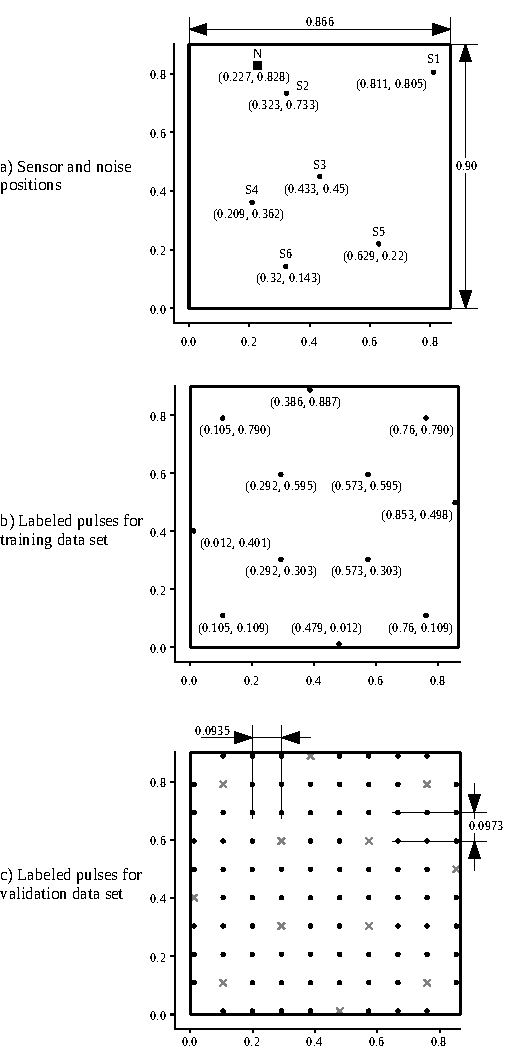
\includegraphics[width=0.5\textwidth]{./chapters/cnn_accelerator/figures/histograms/data_set.pdf}
	\caption{Experimental setup for sensor analytics on structural health monitoring, all lengths are in meters (m).}
	\label{fig:data_set}
\end{figure}

In order to create reproducible acoustic emissions, this demonstration uses 9-cycle sine pulse in a Hanning window with central frequency $f_\mathrm{c}$ (narrow-banded in the frequency domain). This experiment assumes guided Lamb waves based on the plate structure. The narrow-band behavior also reduces the dispersion of the acoustic emission waves~\cite{hannwindowsine}. The waveform can be expressed as a function of time $t$ as follows:

\begin{equation}
x_\mathrm{pulse}(t) = \frac{1}{2} \Big(1-\cos{\frac{f_\mathrm{c} t}{5}} \Big) A_0 \sin{f_\mathrm{c} t}.
\end{equation}

To generate the data sets, slightly different pulse amplitudes and frequencies for excitation are used. The pulse frequency $f_c$ is varied in $\unit[1]{kHz}$ steps between $\unit[300]{kHz}$ and $\unit[349]{kHz}$ and the amplitude $A_0$ is varied in $\unit[0.1]{V}$ steps between $\unit[2.6]{V}$ and $\unit[3.5]{V}$. This produces 500 different pulses for each of the excitation points.

The signals for labeled pulses and noise disturbance are generated by \glspl{awg}. The sensor signals are recorded via a Vallen AMSY-6 measurement system with a resolution of 18 bits and a sampling rate of $f_\mathrm{S} =\unit[10]{MHz}$. The disturbance signal is gaussian noise with amplitudes between 0-3 V. This noise is applied via the piezoelectric device $N$ at $x=\unit[0.227]{m}$ and $y=\unit[0.828]{m}$, see \fig{fig:data_set}(a).

To obtain frequency components, the sampled pulses are converted into the frequency-time domain using the \gls{stft}. This is calculated as follows~\cite{stft_lit}:

\begin{flalign}
\label{stft_eq2}
\mathcal{F}_{m,k}^\gamma= \sum_{n=0}^{N-1} x[n] \cdot \gamma^*[n-m\Delta M]\cdot \mathrm{e}^{\frac{-j 2 \pi k n }{N}}
\end{flalign}

Here $x[n]$ describes a discrete-time signal and $\gamma^*[n-m\Delta M]\cdot \mathrm{e}^{\frac{-j 2 \pi k n }{N}}$ the time- and frequency-shifted window function inside the considered interval $[0 , N-1]$. $\Delta M$ describes the time shift and $N$ the transformation window. Since only discrete frequencies and time points are considered, $m = 0,1,...,M-1$ is valid. For pictorial representation, the magnitude of the complex-valued \gls{stft} is employed in a spectrogram $\mathcal{S}_{m,k}$:

\begin{flalign}
\label{stft_eq3}
\mathcal{S}_{m,k}= \left|\mathcal{F}_{m,k}^\gamma\right|^2 = \left|\sum_{n=0}^{N-1} x[n] \cdot \gamma^*[n-m\Delta M]\cdot \mathrm{e}^{\frac{-j 2 \pi k n }{N}} \right|^2
\end{flalign}

In addition, these spectrograms are scaled in decibels. The spectrogram in decibels $\mathcal{S}_{m,k,\mathrm{dB}}$ produces $\mathcal{S}_{m,k,\mathrm{dB}}= 20 \cdot \mathrm{log}_{10}(\mathcal{S}_{m,k})$. For conversion of data, the experiment uses a signal length of 400 \textmu s (75 \textmu s pretrigger and 325 \textmu s post trigger). Thus, the arrival times of the pulses are included in the spectrogram for all channels and labeled positions. This uses Blackman window function~\cite{blackman_window}, \gls{fft} length of 32 samples, and overlap of 8 samples. The spectrograms are calculated for frequencies in the range of \unit[100]{kHz} to \unit[500]{kHz}. This produces a spectrogram size of 8x16 (8 frequency bins, 16 time values).

In order to generate larger data sets, four further variants are created with time shifts of 15 \textmu s/ 30 \textmu s/ 45 \textmu s/ 60 \textmu s. Subsequently, all spectrograms are converted to grayscale with scaling between \unit[-100]{dB} and \unit[-40]{dB}, see \fig{fig:spectrograms}.

In overall, the data set has a size of 1,440,000 images. This is the result of 500 (pulses) $\cdot$ 5 (spectrograms) $\cdot$ 6 (listening sensors) $\cdot$ 96 (excitation points).

\begin{figure}[t!]
	\centering
	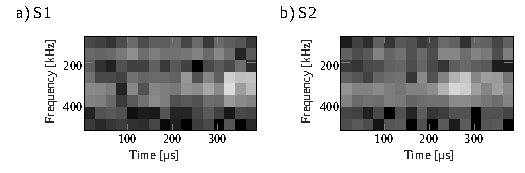
\includegraphics[width=0.5\textwidth]{./chapters/cnn_accelerator/figures/histograms/spectrograms.pdf}
	\caption{Spectrograms of sensors $S_1, S_2$ converted to grayscale for pulses at $x =0.105$ m, $y = 0.109$ m with noise disturbance.}
	\label{fig:spectrograms}
\end{figure}

\subsubsection{CNN-Regression Model}
The data analytics is implemented with a \gls{cnn}-regression model, see \fig{fig:model}. The structure of the model is described below:

\begin{enumerate}[label=\alph*)]
\item Input tensor. This is composed of spectrograms from the sensor signals. The tensor shape is defined by $S \times T \times F$, where $S$ is the number of sensors, and $T \times F$ is the time-frequency resolution of the spectrograms, see \fig{fig:model}(a).

\item Feature extraction. This is composed of three blocks of convolution, batch normalization, and max-pooling layers, see \fig{fig:model}(b). The number of channels in the convolution layers are defined by the hyper-parameters $A$, $B$, and $C$.

\item Regression function. This is an arbitrary function implemented with two fully connected layers and an output layer with linear activation, see \fig{fig:model}(c).
\end{enumerate}


\begin{figure}[t!]
	\centering
	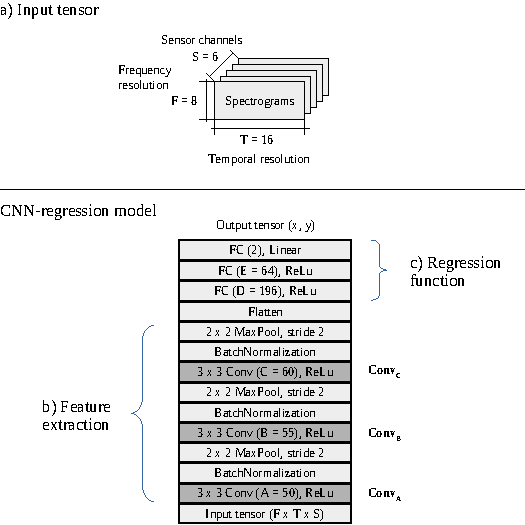
\includegraphics[width=0.5\textwidth]{./chapters/cnn_accelerator/figures/models.pdf}
	\caption{CNN-regression model for sensor analytics.}
	\label{fig:model}
\end{figure}


\subsection{Training}
\subsubsection{Base Model}
The model in \fig{fig:model} is trained using Adam algorithm with iterative search. The Adam optimizer is configured with the default settings presented in \cite{kingma2014adam}: $\alpha = 0.001$, $\beta_1 = 0.9$, $\beta_2 = 0.999$, and $\epsilon = 1\mathrm{e}{-8}$. The training-cycle has a patience of 10 iterations before stop, the optimizer is executed with early stop patience of 10 epochs, and mini-batch size of 512 samples. This is applied using the method described in \Algo{alg:training} with $N_I = 10$, $N_E=10$, $B_{size}=512$.

The training results are illustrated in \fig{fig:optimization}(a). In this optimization, the initial and the final models achieve $MSE=\unit[0.0135]{m^2}$ and $MSE=\unit[0.0122]{m^2}$, respectively. The $MSE$ is calculated with the Euclidean distance (loss) between the real/expected and the predicted/inferred coordinates. The initial model is obtained at the first early stop (after 10 epochs). In each stop, the moving averages of the Adam optimizer get re-initialized. This facilitates searching for better local minima. The model gets saved/updated when finding a better minimum.

\begin{figure}[h!]
	\centering
	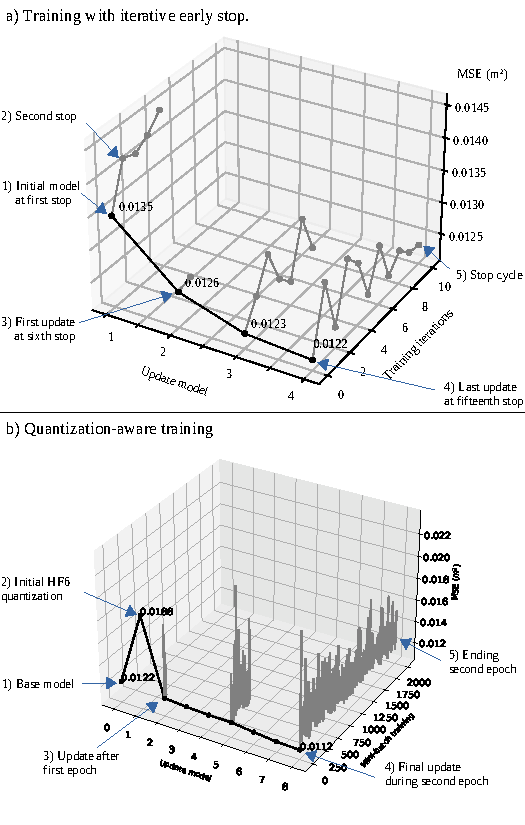
\includegraphics[width=0.5\textwidth]{./chapters/cnn_accelerator/figures/histograms/training_and_quantization.pdf}
	\caption{Training results.}
	\label{fig:optimization}
\end{figure}

The final model achieves $MSE=\unit[0.0122]{m^2}$, which corresponds to $MAE=\unit[0.0955]{m}$. See \fig{fig:model_evaluation}(a). In total, the training takes 379 epochs in 25 cycle-search iterations. The first search takes 43 epochs for the initial model and subsequent search iterations take an average of 14 epochs. The total time is 53 minutes using a \gls{pc} with AMD Ryzen 5 5600H and NVIDIA GeForce RTX 3050 \gls{gpu}.

\begin{figure}[h!]
	\centering
	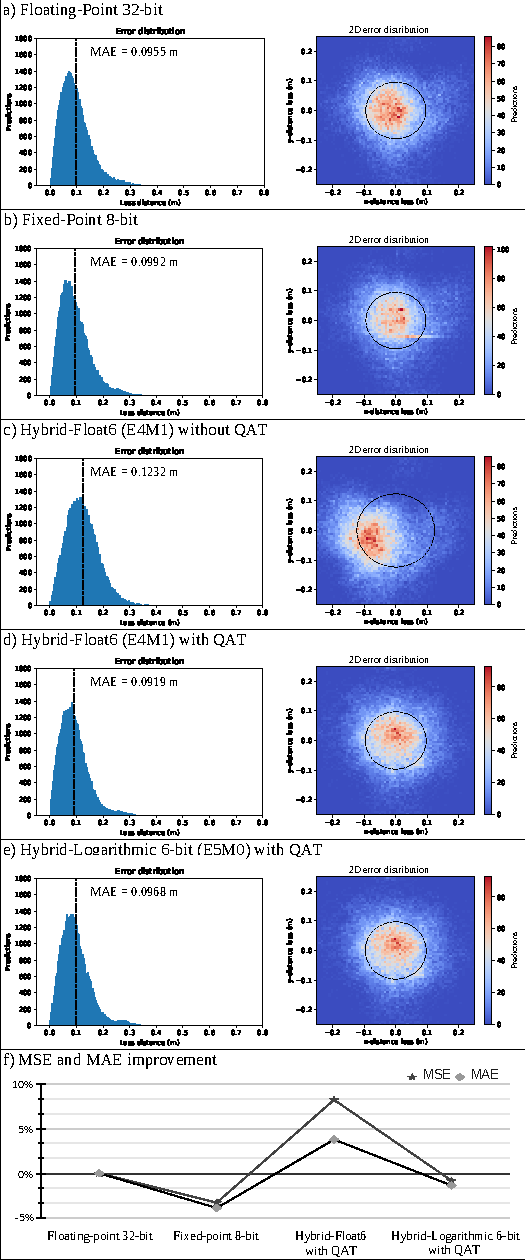
\includegraphics[width=0.5\textwidth]{./chapters/cnn_accelerator/figures/histograms/model_evaluation.pdf}
	\caption{Performance of the model with different data representations.}
	\label{fig:model_evaluation}
\end{figure}

\subsubsection{TensorFlow Lite 8-bit Quantization}
This optimization method converts filter and bias tensors as well as activation maps to 8-bit integer representation, this allows inference using integer-only arithmetic~\cite{hannwindowsine}. In this research, this quantization is applied only to the convolution layers as they are the compute bound operations. Other layers employ 32-bit \gls{fp} representation.

In the compute graph, the input and output feature maps are glued with linear quantization at the input and output of the \emph{Conv2D} operations.

The base model is quantized using the TensorFlow Lite library with integer-only quantization on the \emph{Conv2D} tensor operations. The filter and bias tensors are represented by 8-bit and 32-bit signed integers, respectively. The input and output activation maps are represented by 8-bit signed integer. The TensorFlow quantization includes two additional vectors (output-multiplier and output-shift coefficients), these two vectors are the same shape as the bias vector with 32-bit integer representation.

This model achieves $MSE=\unit[0.0126]{m^2}$ and $MAE=\unit[0.0992]{m}$. See \fig{fig:model_evaluation}(b). The MAE increases 5.1\% of the base model. We attribute this degradation to the 8-bit quantization on the \emph{Conv2D} layers.

\subsubsection{Inference of non-quantized models on HF6 hardware}
To demonstrate backward compatibility, the inference quality of the base model is measured without quantization on the \gls{hf6} hardware. See \fig{fig:model_evaluation}(c). This obtains $MSE=\unit[0.0188]{m^2}$ and $MAE=\unit[0.1232]{m}$. The MAE increases 29.5\% of the base model. We attribute this degradation to the rounding errors of non-quantized filters and bias in \emph{Conv2D} layers.

\subsubsection{Quantization-Aware Training for HF6 hardware}
The \gls{qat} is a post-training optimization. This has been run during two epochs with mini-batch size of 10 samples. This quantization is executed targeting the HF6 format: 4-bit exponent and 1-bit mantissa. This is applied to filter and bias tensors of \emph{Conv2D} layers. This method is described in \Algo{alg:quantization_integration} with $N_{ep}=2$, $B_{size}=10$, $E_{size}=4$, $M_{size}=1$. The optimization results are illustrated in \fig{fig:optimization}(b).

The resulting model achieves $MSE=\unit[0.0112]{m^2}$ and $MAE=\unit[0.0919]{m}$. This corresponds to an error reduction of 8.2\% and 3.77\%, respectively. We attribute this improvement to the regularization effect. See \fig{fig:model_evaluation}(d). The \gls{qat} time is 185 minutes.


\subsubsection{Quantization-Aware Training for Hybrid-Logarithmic 6-bit}
For the sake of quality comparison with logarithmic quantization, the model with 6-bit logarithmic representation is generated. See \fig{fig:floating}(e). This quantization matches the bit size of \gls{hf6}. The filter and bias tensors of \emph{Conv2D} layers are quantized with the 6-bit logarithmic format: 1-bit sign, 5-bit signed exponent, and 0-bit mantissa. This is applied using the method described in \Algo{alg:quantization_integration} with $N_{ep}=2$, $B_{size}=10$, $E_{size}=5$, $M_{size}=0$.

The model achieves $MSE=\unit[0.0123]{m^2}$ and $MAE=\unit[0.0968]{m}$, which correspond to an error increase of 0.82\% and 1.36\%, respectively. We attribute this degradation to the 6-bit logarithmic quantization lacking fractional bits. See \fig{fig:model_evaluation}(e).

A summary of improvement-degradation of MSE and MAE with different data representations is presented in \fig{fig:model_evaluation}(f).

\subsection{Hardware Design Exploration}
The proposed hardware/software co-design is demonstrated on the Zynq-7007S \gls{soc} on the MiniZed development board. This \gls{soc} integrates a single ARM Cortex-A9 \gls{ps} and a \gls{pl} equivalent to Xilinx Artix-7 \gls{fpga} in a single chip~\cite{xilinx2015zynq}. The Zynq-7007S \gls{soc} architecture maps the custom logic and software in the \gls{pl} and \gls{ps}, respectively.

In this platform, the proposed hardware/software architecture is implemented to deploy the sensor analytics application. The desired model is converted to TensorFlow Lite (floating-point) and deployed on the embedded software as a hex dump as a C array. The Zynq-7007S \gls{soc} executes inference with TensorFlow Lite on the \gls{ps}. The computational workload of convolution layers is delegated to the dedicated hardware.

\subsubsection{Benchmark on Embedded CPU}
First, the performance of the embedded \gls{cpu} is explored for inference without hardware acceleration. In this case, TensorFlow Lite creates the \gls{cnn} model as a sequential compute graph executing all computation on the \gls{cpu} (ARM Cortex-A9) at $\unit[666]{MHz}$ with power dissipation of $\unit[1,187]{W}$.

The compute performance and run-time inference of the \gls{cpu} are shown in \Tab{tab:performance}(a) and \fig{fig:runtime}(a), respectively.

\subsubsection{Benchmark on Tensor Processor Synthesized with Xilinx LogiCORE IP for Floating-Point Computation}
For this design, the TP is implemented with standard Xilinx \gls{fp} hardware prior synthesis. The design parameters for the maximum required accelerator on-chip size are:
\begin{itemize}
	\item Max convolution kernel size: $K_W = K_H = 3$.
	\item Max input tensor width: $W_I = 16$.
	\item Max input and output channels: $C_I = 55$, $C_O = 60$.
	\item Filter and bias bit size: $BitSize_F=BitSize_B=32$.
	\item Input tensor bit size: $BitSize_I=32$.
\end{itemize}

Using equations from Section \ref{sec:memory_utilization}, the on-chip memory utilization are $Input_M=84,480$b, $Filter_M=950,400$b, and $Bias_M=1,920$b. Hence, the required on-chip memory buffer size is $TP_B=1,036,800$b.

The post-implementation resource utilization and power dissipation are presented in \Tab{tab:resource_utilization}(a). The complete hardware platform utilizes 83\% of BRAM, this includes the on-chip memory requirements of the \gls{tp}, \gls{dma}, and AXI interconnects. The total available on-chip memory (BRAM) on the Zynq-7007S \gls{soc} is $\unit[1.8]{Mb}$. After hardware syntheses, the estimated power dissipation of the \gls{tp} is $\unit[85]{mW}$ at $\unit[200]{MHz}$ (this estimation is provided by Xilinx Vivado).

\begin{table}[!h]\centering
	\caption{Resource utilization and power dissipation on the Zynq-7007S SoC.}\label{tab:resource_utilization}
	\scriptsize
	\begin{tabular}{lrrrrrr}\toprule
		\multirow{2}{*}{\textbf{TP engine}} &\multicolumn{4}{c}{\textbf{Post-implementation resource utilization}} &\multirow{2}{*}{\textbf{Power (W)}} \\\cmidrule{2-5}
		&\textbf{LUT} &\textbf{FF} &\textbf{DSP} &\textbf{BRAM 36Kb} & \\\midrule
		\multirow{2}{*}{(a) Floating-Point} &5,578 &8,942 &23 &41.5 &\multirow{2}{*}{1.429} \\
		&39\% &31\% &35\% &\textbf{83\%} & \\
		\multirow{2}{*}{(b) Hybrid-Float6} &7,313 &10,330 &20 &15 &\multirow{2}{*}{1.424} \\
		&51\% &36\% &30\% &\textbf{30\%} & \\
		\bottomrule
	\end{tabular}
\end{table}

The compute performance and inference schedule of the model on this hardware implementation are shown in \Tab{tab:performance}(b) and \fig{fig:runtime}(b), respectively. During run-time, the software (TensorFlow Lite) delegates computation to the \gls{tp} as dedicated hardware for \emph{Conv2D} tensor operations.

The implementation of the dot-product with standard \gls{fp} engine (IEEE 754 arithmetic) utilizes proprietary multiplier and adder floating-point operator cores. Vivado \gls{hls} implements \gls{fp} arithmetic operations by mapping them onto Xilinx LogiCORE IP cores, these \gls{fp} operator cores are instantiated in the resultant \gls{rtl}~\cite{hrica2012floating}. In this case, the implementation of the dot-product with the standard \gls{fp} computation reuses the multiplier and adder cores in different compute sections of the \gls{tp}. The post-implementation resource utilization and power dissipation of the individual floating-point operator cores are shown in \Tab{tab:LogiCORE}.

\begin{table}[!t]\centering
	\caption{Compute performance of the CPU and TP on each Conv2D tensor operation. This table presents: tensor operation, computational cost in mega floating-point operations (MFLOP), latency, throughput, power efficiency, and estimated energy consumption as the energy delay product (EDP).}\label{tab:performance}
	\scriptsize
	\begin{tabular}{lrrrrrr}\toprule
		\textbf{Operation} &\textbf{MFLOP} &\textbf{t (ms)} &\textbf{MFLOP/s} &\textbf{MFLOP/s/W} &\textbf{EDP (mJ)} \\\midrule
		& &\multicolumn{4}{l}{\textbf{a) CPU (ARM Cortex-A9) @666MHz, 1.187 W}} \\
		Conv\textsubscript{A} &0.691 &112.24 &6.16 &5.19 &133.23 \\
		Conv\textsubscript{B} &1.584 &213.13 &7.43 &6.26 &252.99 \\
		Conv\textsubscript{C} &0.475 &46.59 &10.20 &8.59 &55.31 \\
		& &\multicolumn{4}{l}{\textbf{b) TP (Floating-Point engine) @200MHz, 85 mW}} \\
		Conv\textsubscript{A} &0.691 &12.49 &55.34 &651.11 &1.06 \\
		Conv\textsubscript{B} &1.584 &16.39 &96.66 &1,137.20 &1.39 \\
		Conv\textsubscript{C} &0.475 &3.59 &132.44 &1,558.13 &0.30 \\
		& &\multicolumn{4}{l}{\textbf{c) TP (Hybrid-Float6 engine) @200MHz, 84 mW}} \\
		Conv\textsubscript{A} &0.691 &6.92 &99.81 &1,188.24 &0.58 \\
		Conv\textsubscript{B} &1.584 &4.41 &358.94 &4,273.09 &0.37 \\
		Conv\textsubscript{C} &0.475 &0.99 &482.44 &5,743.29 &0.08 \\
		\bottomrule
	\end{tabular}
\end{table}

\begin{figure}[t!]
	\centering
	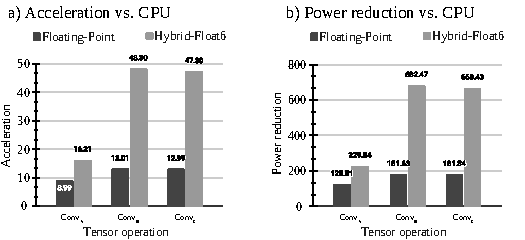
\includegraphics[width=0.5\textwidth]{./chapters/cnn_accelerator/figures/power_breakdown/acceleration_power_reduction.pdf}
	\caption{Inference acceleration and power reduction on the TP with floating-point and HF6 vs. CPU on the Zynq-7007S SoC.}
	\label{fig:acceleration}
\end{figure}


\begin{table}[!h]\centering
	\caption{Resource utilization and power dissipation of individual multiplier and adder floating-point (IEEE 754) operator cores (Xilinx LogiCORE IP).}\label{tab:LogiCORE}
	\scriptsize
	\begin{tabular}{lrrrrrr}\toprule
		\textbf{Core operation} &\textbf{DSP} &\textbf{FF} &\textbf{LUT} &\textbf{Latency (clk)} &\textbf{Power (mW)} \\\midrule
		Multiplier &3 &151 &325 &4 &7 \\
		Adder &2 &324 &424 &8 &6 \\
		\bottomrule
	\end{tabular}
\end{table}



\subsubsection{Tensor Processor Synthesized with Hybrid-Float6 Hardware Architecture}
To demonstrate the proposed design, the \gls{tp} with \gls{hf6} hardware reuses the standard \gls{fp} design parameters with the following variation for the 6-bit representation in filter and bias: $BitSize_F=BitSize_B=6$.

Using equations from Section \ref{sec:memory_utilization}, the on-chip memory requirements for the hardware accelerator are $Input_M=\unit[84,480]{b}$, $Filter_M=\unit[178,200]{b}$, $Bias_M=\unit[360]{b}$. Hence, the required on-chip memory buffer size is $TP_B=\unit[263,040]{b}$.

The post-implementation resource utilization and power dissipation are presented in \Tab{tab:resource_utilization}(b). The complete hardware platform utilizes 30\% of BRAM, this includes the on-chip memory requirements of the \gls{tp}, \gls{dma}, and AXI interconnects. The estimated power dissipation of the \gls{tp} is $\unit[84]{mW}$ at $\unit[200]{MHz}$ (this estimation is provided by Xilinx Vivado).

The compute performance and inference schedule of the model on this hardware implementation are shown in \Tab{tab:performance}(c) and \fig{fig:runtime}(c), respectively. \Fig{fig:acceleration} presents a comparison of the acceleration and the reduction of power dissipation between standard \gls{fp} and \gls{hf6} hardware implementations.

This deployment does not require model treatment for hardware compatibility. For backward compatibility, the 6-bit \gls{fp} representation is wrapped into the standard \gls{fp}. The dedicated hardware design extracts the 6-bit format automatically to perform computation.

\begin{figure}[t!]
	\centering
	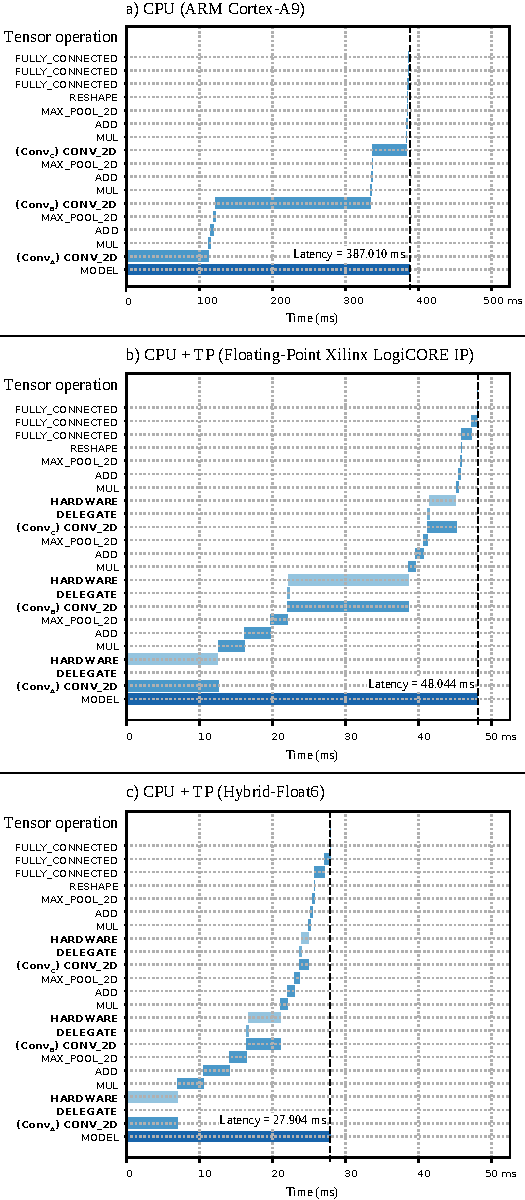
\includegraphics[width=0.5\textwidth]{./chapters/cnn_accelerator/figures/runtime/runtime.pdf}
	\caption{Run-time inference of TensorFlow Lite on the Zynq-7007S SoC. (a) CPU ARM Cortex-A9 at $\unit[666]{MHz}$, (b) cooperative CPU + TP with floating-point Xilinx LogiCORE IP at $\unit[200]{MHz}$, and (c) cooperative CPU + TP with Hybrid-Float6 at $\unit[200]{MHz}$.}
	\label{fig:runtime}
\end{figure}

\subsection{Discussion}
\subsubsection{Training and Quantization}
The training with iterative early stop obtains a model with enhanced accuracy than standard early stop. This method iteratively resets the moving averages of Adam's optimizer, which helps to iteratively search for better local minima. This iterative search is suitable for models with low computational cost.

The TensorFlow Lite 8-bit quantization preserves the overall model accuracy. In some cases, the associated regularization effect can improve the accuracy. However, the error distribution in \gls{cnn} linear regressions gets slightly degraded. In particular, 8-bit quantized output layers incur in discrete-degradation patterns, \fig{fig:2d_error_distribtion}(b) shows this effect on three different models. Vertical and horizontal patterns appear in the error distribution of 8-bit fixed-point quantization. We attribute this effect to the 8-bit resolution in the activation maps. In the case of \gls{hf6} quantization, the activation maps are represented by floating-point preventing this degradation.

The proposed 6-bit \gls{fp} representation (E4M1) improves latency, hardware area, and power dissipation, while preserving model accuracy. For comparison, in our application, this number format produces better results than the 6-bit logarithmic representation (E5M0). This is demonstrated in \Fig{fig:model_evaluation}(d) and \Fig{fig:model_evaluation}(e).

In \cite{lai2017deep}, Lai et al. demonstrated that 4-bit exponent and X-bit mantissa preserves accuracy on SqueezeNet, AlexNet, GoogLeNet, and VGG-16. To contribute on this, I investigated 4-bit exponent and 1-bit mantissa to ALL-CNN-C~\cite{springenberg2014striving}, this produces an accuracy degradation of 1.39\% and 0.11\% with \gls{qat}. While applying 6-bit logarithmic produces a degradation of 11.18\% and 7.22\% with \gls{qat}.

\begin{figure}[t!]
	\centering
	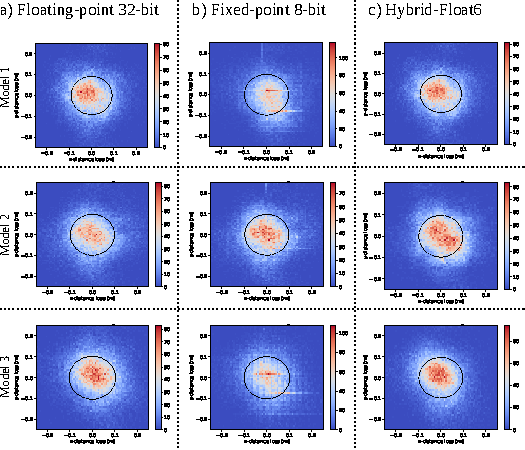
\includegraphics[width=0.5\textwidth]{./chapters/cnn_accelerator/figures/histograms/2D_error_distribtion.pdf}
	\caption{2D error distribution of three CNN-regression models.}
	\label{fig:2d_error_distribtion}
\end{figure}

\subsubsection{Implementation and Performance}
The proposed \gls{hf6} implementation reduces on-chip memory and \gls{dsp} utilization while slightly increasing \glspl{ff} and \glspl{lut} compared to the standard \gls{fp} implementation. See \Tab{tab:resource_utilization} and \Fig{fig:resource_utilization}. This is attributed to the \gls{hf6} logic implementation using \gls{ff} and \gls{lut}, while the \gls{fp} logic implementation uses Xilinx LogiCORE IPs mainly with \glspl{dsp}.

The compute performance of the \gls{cpu} and \gls{tp} on each convolution layer is presented in \Tab{tab:performance} and \fig{fig:acceleration}. 
The peak acceleration and power efficiency of the \gls{tp} with standard \gls{fp} (Xilinx LogiCORE IP) is $13\times$ and \unit[1,558.13]{MFLOPS/s/W}, respectively. While the peak acceleration and power efficiency of the \gls{tp} with \gls{hf6} is $48.3\times$ and \unit[5,743.29]{MFLOPS/s/W}, respectively. The \gls{hf6} hardware demonstrates an improvement of $3.7\times$ in acceleration and power efficiency with respect to the standard \gls{fp} hardware. See \Fig{fig:acceleration}.

The estimated power dissipation on the \gls{soc} is presented in \fig{fig:power}. This shows a very similar breakdown of power dissipation in both implementations. However, the energy efficiency is increased due to the reduced latency in \gls{hf6} hardware. A comparison of related work is presented in \Tab{tab:comparison}.

\begin{figure}[h!]
	\centering
	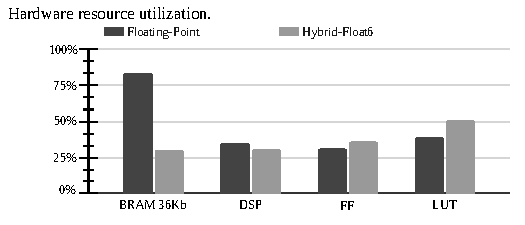
\includegraphics[width=0.5\textwidth]{./chapters/cnn_accelerator/figures/power_breakdown/resource_utilization.pdf}
	\caption{Hardware resource utilization on the Zynq-7007S SoC.}
	\label{fig:resource_utilization}
\end{figure}

\begin{figure}[h!]
	\centering
	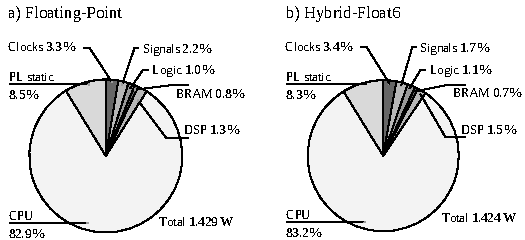
\includegraphics[width=0.5\textwidth]{./chapters/cnn_accelerator/figures/power_breakdown/power_breakdown.pdf}
	\caption{Estimated power dissipation on the Zynq-7007S SoC with PS at $\unit[666]{MHz}$ and PL at $\unit[200]{MHz}$.}
	\label{fig:power}
\end{figure}

The run-time inference of TensorFlow Lite on the \gls{soc} is illustrated in \Fig{fig:runtime}. This shows the convolution layers as the compute-bound operations. The proposed embedded platform is a cooperative system where the convolution operations are delegated to the dedicated hardware accelerator. The ARM \gls{cpu} obtains a latency of \unit[387]{ms} (\unit[2.58]{FPS}). The platform with standard \gls{fp} hardware obtains a latency of \unit[48]{ms} (\unit[20.8]{FPS}), while the implementation with \gls{hf6} obtains a latency of \unit[27.9]{ms} (\unit[35.84]{FPS}). These represent an overall acceleration of $8\times$ and $13.87\times$ over the \gls{cpu}, respectively.

This design facilitates \gls{ml} compatibility/portability as the 6-bit \gls{fp} is wrapped in the standard \gls{fp} representation. The dedicated hardware design extracts the 6-bit format automatically and performs computation.

\subsubsection{SoC Design and Compatibility}
The proposed design is an alternative for high accuracy and low-power floating-point inference. The system runs as a cooperative hardware/software mechanism. This architecture delegates compute-bound tensor operations to a hardware accelerator.

The hybrid 32-bit \gls{fp} and 6-bit \gls{fp} quantization enables high quality of results and backward \gls{ml} compatibility. Backwards \gls{ml} compatibility gives portability from training to inference. This enables to run inference of \gls{hf6} quantized models on standard \gls{fp} hardware and vise versa. The proposed \gls{hf6} architecture allows to compute inference of non-quantized floating-point \gls{ml} models for rapid deployment; however, this will incur in accuracy degradation depending on the resilience of the model, see \Fig{fig:model_evaluation}(c).

\begin{table*}[!t]\centering
	\caption{Comparison of hardware implementation with related work.}\label{tab:comparison}
	\scriptsize
	\begin{tabular}{lrrrrrr}\toprule
		Platform &Chunsheng et al. \cite{mei2017200mhz} &Chen et al. \cite{wu2021low} &BFP \cite{lian2019high} &Paolo et al. \cite{meloni2019cnn} &This work \\\midrule
		Device &XC7VX690T &XC7K325T &XC7VX690T &XC7Z007S &XC7Z007S \\
		Year &2017 &2019 &2019 &2019 &2023 \\
		Dev. kit cost &\$7,494 &\$1,299 &\$7,494 &\$89 &\$89 \\
		Format (activation/weight) &FP 16-bit &FP 8-bit / 8-bit &FP 16-bit / 8-bit &INT 16-bit &FP 32-bit / 6-bit \\
		Frequency (MHz) &200 &200 &200 &80 &200 \\
		Peak power efficiency (GFLOP/s/W) &18.72 &115.40 &82.88 &2.98 &5.74 \\
		Peak throughput (GFLOP/s) & 202.42 & 1086.8 & 760.83 &  10.62& 0.482\\
		Wall plug power (W) &10.81 &9.42 &9.18 &2.5 &\textbf{2.3} \\
		BRAM 36Kb utilization &196.5 &234.5 &913 &44 &\textbf{15} \\
		DSP utilization &1728 &768 &1027 &54 &\textbf{20} \\
		\bottomrule
	\end{tabular}
\end{table*}